\documentclass{article}
\usepackage{fullpage}
\usepackage{color}
\usepackage[normalem]{ulem}
\usepackage{hyperref}
\usepackage{enumitem}
\usepackage{graphicx}
\hypersetup{colorlinks}
\hyphenpenalty=100000
\begin{document}

\setlength{\voffset}{3.5in}
\title{M1}
\author{\Large Team Sriroku\\
Tom Atnip, George Mammarella, Jeremy Tramm}
\date{\today}
\maketitle
\clearpage
\setlength{\voffset}{0pt}
\tableofcontents
\clearpage


\begin{Large}
\textbf{Changes}
\end{Large}
\\

\begin{tabular}{ | p{1.5in} | p{4.5in} | }
\hline
\textbf{Date} & \textbf{Description}\\
\hline
\hline
March 13, 2013 & Document started\\
\hline
\hline
March 14, 2013 & Added image to document. \\
\hline
\end{tabular}
\clearpage

\section{High Level Problem Statement}
The program will be a standalone desktop application that allows users to play the game of Sudoku. The game will support a couple different variations of the game along with varying levels of difficulty. The game will be developed using the test driven development approach, and will follow a (to be determined) scale of test completeness. 

\section{The Game}

\begin{center}
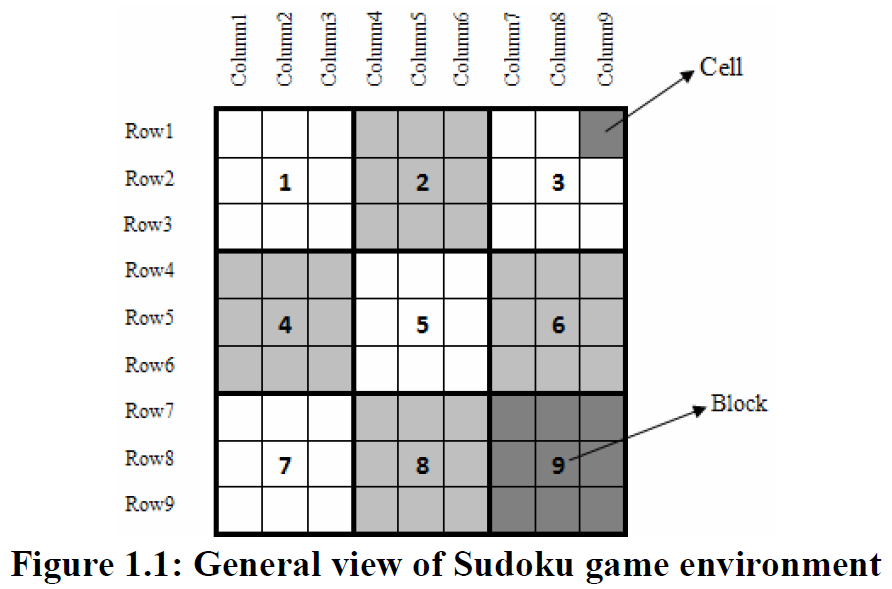
\includegraphics[scale=0.5]{SudokuBoard.png}
\end{center}

\subsection{How to play}
The board is defined by cell, block, row, and column as Figure 1.1 illustrates. The whole board is actually a 9-by-9 grid made of nine smaller 3-by-3 grids called blocks. The smallest square in the traditional game is called a cell which contains a number, ranging from 1 to 9, or is empty signifying empty. Our application will allow users to store multiple guesses per cell block. The board is composed of rows and columns from top-left corner.

\subsection{Goal}
The game starts with a grid that has some of the cells already filled, known as givens. The object of the game is to place a digit from 1 to 9 into each cell of the grid. However each digit can only be used once in each row, each column, and each block. Additionally, all the nine rows, nine columns and nine blocks are required to contain all the digits from 1 through 9. These limitations for placing digits in three locations are respectively called row constraint, column constraint and block constraint.

\section{Features}

\begin{tabular}{ | p{1.5in} | p{4.5in} | }
\hline
\textbf{Feature Number} & \textbf{Description}\\
\hline
\hline
F00 & The application will allow the user to play the game while following a given set of rules based on the version of the game that they have chosen.\\
\hline
F01 & The game will support multiple versions of play that are variations of the basic game but include new rules or board layout.\\
\hline
F02 & The application will support localization, supporting at least two languages.\\
\hline
F03 & There will be support for allowing users to ask for the application to solve part of or the rest of the puzzle for them.\\
\hline
F04 & The user will be able to choose a level of difficulty to play at.\\
\hline
F05 & The user will be able to save their current game state for continuing later on.\\
\hline
F06 & The system will create puzzles for play as the user requests new ones, puzzles will not be pre-stored.\\
\hline
F07 & Cells will be able to hold multiple guesses.\\
\hline
F08 & If a player confirms a cell, other cells with multiple guesses that conflict with the confirmed number will be automatically removed.\\
\hline
F09 & The game will highlight cells that break game constraints.\\
\hline
\end{tabular}

\section{Framework and Technology}
Using Java 1.7 and JUnit 4.

\end{document}